%% This is file `DEMO-TUDaThesis.tex' version 1.20-beta (2019/10/21),
%% it is part of
%% TUDa-CI -- Corporate Design for TU Darmstadt
%% ----------------------------------------------------------------------------
%%
%%  Copyright (C) 2018--2019 by Marei Peischl <marei@peitex.de>
%%
%% ============================================================================
%% This work may be distributed and/or modified under the
%% conditions of the LaTeX Project Public License, either version 1.3c
%% of this license or (at your option) any later version.
%% The latest version of this license is in
%% http://www.latex-project.org/lppl.txt
%% and version 1.3c or later is part of all distributions of LaTeX
%% version 2008/05/04 or later.
%%
%% This work has the LPPL maintenance status `maintained'.
%%
%% The Current Maintainers of this work are
%%   Marei Peischl <tuda-ci@peitex.de>
%%   Markus Lazanowski <latex@ce.tu-darmstadt.de>
%%
%% The development respository can be found at
%% https://github.com/tudace/tuda_latex_templates
%% Please use the issue tracker for feedback!
%%
%% ============================================================================
%%
% !TeX program = lualatex
%%

\documentclass[
	ngerman,
	ruledheaders=section,%Ebene bis zu der die Überschriften mit Linien abgetrennt werden, vgl. DEMO-TUDaPub
	class=report,% Basisdokumentenklasse. Wählt die Korrespondierende KOMA-Script Klasse
	thesis={type=bachelor},% Dokumententyp Thesis, für Dissertationen siehe die Demo-Datei DEMO-TUDaPhd
	accentcolor=9c,% Auswahl der Akzentfarbe
	custommargins=geometry,% Ränder werden mithilfe von typearea automatisch berechnet
	marginpar=false,% Kopfzeile und Fußzeile erstrecken sich nicht über die Randnotizspalte
	BCOR=10mm,%Bindekorrektur, falls notwendig
	parskip=half-,%Absatzkennzeichnung durch Abstand vgl. KOMA-Sript
	fontsize=11pt,%Basisschriftgröße laut Corporate Design ist mit 9pt häufig zu klein
	colorback=false, % Schaltet zwischen dem farbigen Block auf der Titelseite und weißem Hintergrund um
	bibliography=totoc, % bibliography in toc
	listof=totoc % list of X in toc
%	logofile=example-image, %Falls die Logo Dateien nicht vorliegen
]{tudapub}

%change margins
\geometry{a4paper}


% Der folgende Block ist nur bei pdfTeX auf Versionen vor April 2018 notwendig
\usepackage{iftex}
\ifPDFTeX
\usepackage[utf8]{inputenc}%kompatibilität mit TeX Versionen vor April 2018
\fi

%%%%%%%%%%%%%%%%%%%
%Sprachanpassung & Verbesserte Trennregeln
%%%%%%%%%%%%%%%%%%%
\usepackage[english, main=english]{babel}
\usepackage[autostyle]{csquotes}% Anführungszeichen vereinfacht
\usepackage{microtype}


%%%%%%%%%%%%%%%%%%%
%Literaturverzeichnis
%%%%%%%%%%%%%%%%%%%
\usepackage{biblatex}   % Literaturverzeichnis
\bibliography{bibliography}


%%%%%%%%%%%%%%%%%%%
%Tabellen
%%%%%%%%%%%%%%%%%%%
%\usepackage{array}     % Basispaket für Tabellenkonfiguration, wird von den folgenden automatisch geladen
\usepackage{tabularx}   % Tabellen, die sich automatisch der Breite anpassen
%\usepackage{longtable} % Mehrseitige Tabellen
%\usepackage{xltabular} % Mehrseitige Tabellen mit anpassarer Breite
\usepackage{booktabs}   % Verbesserte Möglichkeiten für Tabellenlayout über horizontale Linien
\usepackage{multirow}
\usepackage{ltablex} % combine the features of the tabularx package (auto-sized columns in a fixed width table) with those of the longtable package (multi-page tables).

%%%%%%%%%%%%%%%%%%%
% Custom packages
%%%%%%%%%%%%%%%%%%%
%\usepackage{mathtools} % erweiterte Fassung von amsmath
%\usepackage{amssymb}   % erweiterter Zeichensatz
%\usepackage{siunitx}   % Einheiten
\usepackage[center,labelfont=bf]{caption}
\usepackage{subfig} % make it possible to include more than one captioned figure/table in a single float
\usepackage{graphicx} % support the \includegraphics command and options
\usepackage{array} % for better arrays (eg matrices) in maths
\usepackage{paralist} % very flexible & customisable lists (eg. enumerate/itemize, etc.)
\usepackage{verbatim} % adds environment for commenting out blocks of text & for better verbatim
\usepackage{float}
\usepackage{amsmath}
\usepackage{acronym}

\usepackage{hyperref} % Hyperlinks
\usepackage[toc]{appendix} % Appendices (also shown in toc)
\usepackage{amsthm} %Typesetting theorems

\usepackage[linesnumbered,ruled]{algorithm2e}
\usepackage{enumitem}

\usepackage{blindtext} % to generate dummy text for the example

% sets the default path for images
\graphicspath{{img/}}

%Formatierungen für Beispiele in diesem Dokument. Im Allgemeinen nicht notwendig!
\let\file\texttt
\let\code\texttt

\begin{document}

\Metadata{
	title=Example Title of your Thesis,
	author=Max Mustermann
}

\title{Example Title of your Thesis}
\subtitle{}
\author[Signature]{Max Mustermann}%optionales Argument ist die Signatur, 
\reviewer{Prof. Dr. Carsten Binnig \and Gutachter 2}%Gutachter

%Diese Felder erden untereinander auf der Titelseite platziert. 
%\department ist eine notwendige Angabe, siehe auch dem Abschnitt `Abweichung von den Vorgaben für die Titelseite'
\department{inf} % Das Kürzel wird automatisch ersetzt und als Studienfach gewählt, siehe Liste der Kürzel im Dokument.
\institute{Data Management Lab}
\addTitleBoxLogo{dm_logo}
\submissiondate{\today}
\examdate{\today}

%	\tuprints{urn=1234,printid=12345}
%	\dedication{Für alle, die \TeX{} nutzen.}

\maketitle

% erzeugt eine Selbstständigkeitserklärung mit Unterschriftenzeile.
\affidavit

% insert abstract before contents
\begin{abstract}
    
Write a short summary of your thesis.
\blindtext

\end{abstract}







% create the table of contents
\tableofcontents

% List of figures (Abbildungsverzeichnis):
\listoffigures


\chapter*{List of Abbreviations}
\addcontentsline{toc}{chapter}{List of Abbreviations}

\begin{acronym}
\acro{API}{Ap\-pli\-ca\-tion Programming Interface}		
\acro{CQ}{Completion Queue}		
\acro{DBMS}{Database Management System}		
\acro{DMA}{Direct Memory Access}
\acro{HPC}{High Performance Computing}
\acro{IB}{InfiniBand}
\acro{MPI}{Message Passing Interface}
\acro{NIC}{Network Interface Controller}		
\acro{OLAP}{On-line Analytical Processing}		
\acro{OLTP}{On-line Transactional Processing}		
\acro{QP}{Queue Pair}		
\acro{RAM}{Random Access Memory}		
\acro{RDMA}{Remote Direct Memory Access}		
\acro{RNIC}{RDMA-enabled Network Interface Controller}		
\acro{RoCE}{RDMA over Converged Ethernet}		
\acro{RQ}{Receive Queue}		
\acro{RR}{Receive Request}	
\acro{SDN}{Software Defined Networking}
\acro{SQ}{Send Queue}		
\acro{SR}{Send Request}		
\acro{TLB}{Translation Lookaside Buffer}
\acro{TCP/IP}{Transmission Control Protocol/Internet Protocol}	
\end{acronym}
\chapter{Introduction}
\label{chap:introduction}
\IMRADlabel{introduction} % Mechanismus um das Strukturierungsmodell IMRaD zu kennzeichnen
% Recipe for a good introduction (LeanStore)
    %How are things done before new HW (pre main-memory db)
    %Motivate why the way it was done is suboptimal
    %Visually illustrate the suboptimality
    %Include related approaches and state suboptimality
    %Motivate further by hardware trends
    %Raise fundamental question for paper
    %Give short overview of contribution and result (abstract-like)


\section{Context and Motivation}
\label{sec:context}
This is a dummy citation \cite{6651094}.
And this is an example of using an acronym which was defined previously \ac{RDMA}.
The long form of the acronym is only used the first time, the short form is \ac{RDMA}.

\blindtext

\section{Problem Statement}
\label{sec:problemStatment}

\section{Goals and Contributions}
\label{sec:goals}

\section{Thesis Outline}
\label{sec:outline}
Describe what the thesis contains

\chapter{Background}
\label{chap:background}
In order to grant a better understanding of the subsequent chapters, this chapter is going to provide a background to the terms and concepts used in the thesis\dots

\section{Remote Direct Memory Access (RDMA)}
\label{sec:RDMA}
\ac{RDMA} is an alternative to the traditional \ac{TCP/IP} network communication protocols. In short, \ac{RDMA} can provide access to a remote machine's memory without performing unnecessary intermediate copies of the memory while also bypassing the CPU of the remote machine.\\
RDMA has been gaining traction in the academic community (Figure \ref{fig:rdmaHits}). This growing popularity is because \ac{RDMA} overcomes some limitations by \ac{TCP/IP}, and by doing so, helps to provide high bandwidth and low latency.
Therefore, in order to explain \ac{RDMA}, the shortcomings of \ac{TCP/IP} socket programming is stated, and thus motivating the benefit of \ac{RDMA}.

\begin{figure}[h]
  \centering
  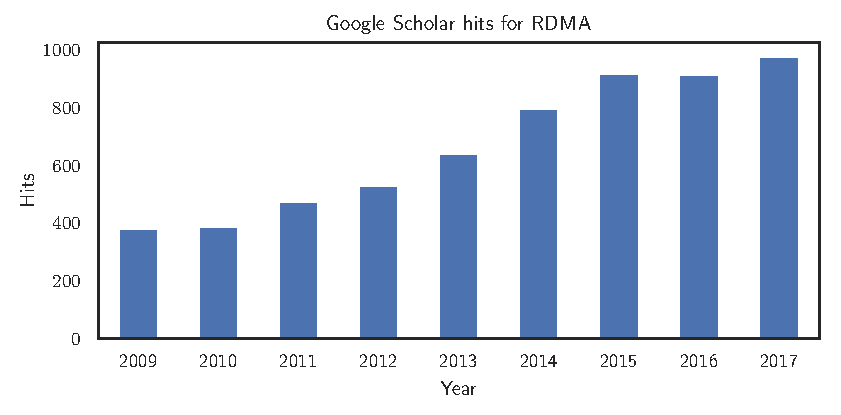
\includegraphics[width=0.7\linewidth]{GoogleScholarRDMAHits.pdf}
  \caption{Google Scholar hits of RDMA keyword}
  \label{fig:rdmaHits}
\end{figure}
\chapter{Design}
\label{chap:design}
\IMRADlabel{methods} % Mechanismus um das Strukturierungsmodell IMRaD zu kennzeichnen

This chapter presents the design behind\dots

\section{Requirement Analysis}
\label{sec:requirements}

In order to better understand the requirements, the different trends in\dots
\blindtext
\chapter{Implementation}
\label{chap:implementation}
Explain how the concepts you developed where implemented. Focus on interesting/challenging details.

\section{Implementation Overview}
\label{sec:implementationOverview}
\blindtext
\chapter{Evaluation}
\label{chap:evaluation}
\IMRADlabel{results} % Mechanismus um das Strukturierungsmodell IMRaD zu kennzeichnen

To evaluate the performance and usefulness of\dots

\section{Experimental setup}
\label{sec:experimentalSetup}
\blindtext

\chapter{Conclusion and Future Work}
\label{chap:conclusion_futurework}
\IMRADlabel{discussion} % Mechanismus um das Strukturierungsmodell IMRaD zu kennzeichnen

This chapter first summarizes and concludes the contributions of this thesis by presenting the strengths behind the design concepts and concluding upon the evaluation. Following, an outlook of research challenges for future work is given.


\section{Conclusion}
\label{sec:conclusion}
Mirror the contributions given in intro. 

Conclude on the evaluation 
\blindtext

\section{Future Work}
\label{sec:future_work}
\blindtext
		
\printbibliography


\begin{appendices}

\addtocontents{toc}{\protect\setcounter{tocdepth}{1}}
\makeatletter
\addtocontents{toc}{%
  \begingroup
  \let\protect\l@chapter\protect\l@section
  \let\protect\l@section\protect\l@subsection
}

\chapter{Experiment Parameters}
\label{appendix:experiment_parameters}
The experiments conducted in the \nameref{chap:evaluation} Chapter were executed with the following DPI parameters. Note, an \textit{x} indicates the parameter has been varied for the experiment.

%segment size, ring size, internal buffer size
\begin{tabular}{|l|c|c|c|c|}
    \hline
     & Message size & Segment size & Ring size (segments) & Internal output buffer size \\
    \hline
    Exp. A & \textit{x} & 64 MiB & 10 & 8 MiB \\
    Exp. B & \textit{x} & \textit{x} & 100 & 4 MiB \\
    Exp. C & 4 KiB & 64 MiB & 10 & \textit{x} \\
    Exp. D & 4 KiB & 32 MiB & \textit{x} & 4 MiB \\
    Exp. E & 4 KiB & \textit{x} & \textit{x} & 4 MiB \\
    Exp. F & \textit{x} & 32 MiB & 50 & 8 MiB \\
    Exp. G & \textit{x} & 64 MiB & 50 & 4 MiB \\
    Exp. H & 8 KiB & 4 MiB & \textit{x} & 2 MiB \\
    \hline
\end{tabular}



\end{appendices}
	
\end{document}
